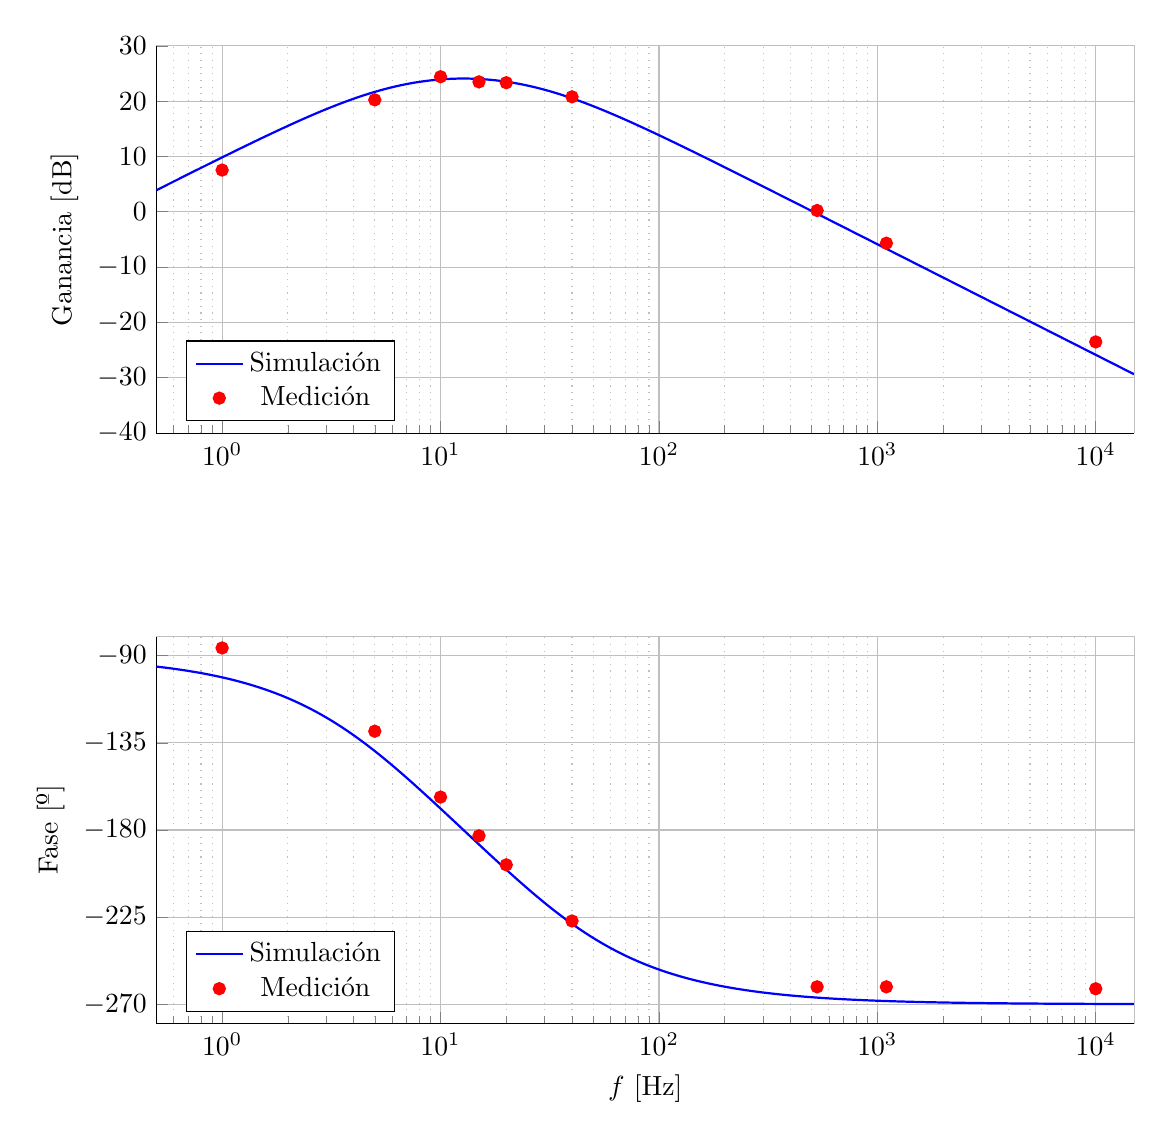
\begin{tikzpicture}
    \pgfplotsset{
        nice plot/.style={
            /pgf/number format/read comma as period,
            grid=both,
            major grid style={solid, gray!50},
            minor grid style={dotted, gray!50},
            axis line style={black},
            axis x line* = bottom,
            axis y line* = left,
            extra description/.code={
                \draw[gray!50] (rel axis cs:0,1) -- (rel axis cs:1,1) -- (rel axis cs:1,0);
            },
            width=14cm,
            height=6.5cm,
            xmin=0.5, xmax=15000,
            minor x tick num=9,
            minor y tick num=0,
        }
    }

    \begin{semilogxaxis}[
        nice plot,
        ylabel={Ganancia [dB]},
        ymin=-40, ymax=30,
        ytick={-40, -30, -20, -10, 0, 10, 20, 30},
        legend pos=south west,
    ]
        % Graficamos la magnitud ideal en dB (Simulación)
        \addplot[thick, blue, domain=0.5:15000, samples=300] {
            20*log10(3200 * 2 * pi * x) - 10*log10((2 * pi * x)^2 + 1600) - 10*log10((2 * pi * x)^2 + 25600)
        };
        \addlegendentry{Simulación}

        % Puntos medidos
        \addplot[only marks, mark=*, red, thick] coordinates {
            (1, 7.54)
            (5, 20.23)
            (10, 24.41)
            (15, 23.48)
            (20, 23.33)
            (40, 20.78)
            (530, 0.23)
            (1100, -5.68)
            (10000, -23.52)
        };
        \addlegendentry{Medición}
    \end{semilogxaxis}

    \begin{semilogxaxis}[
        nice plot,
        xlabel={$f$ [Hz]},
        ylabel={Fase [º]},
        ymin=-280, ymax=-80,
        ytick={-270, -225, -180, -135, -90},
        at={(0,-7.5cm)},
        legend pos=south west,
    ]
        % Graficamos la fase ideal en grados
        \addplot[thick, blue, domain=0.5:15000, samples=300] {
            -90 - atan(2 * pi * x / 40) - atan(2 * pi * x / 160)
        };
        \addlegendentry{Simulación}

        % Puntos medidos
        \addplot[only marks, mark=*, red, thick] coordinates {
            (1, -86)
            (5, -129)
            (10, -163)
            (15, -183)
            (20, -198)
            (40, -227)
            (530, -261)
            (1100, -261)
            (10000, -262)
        };
        \addlegendentry{Medición}
    \end{semilogxaxis}
\end{tikzpicture}
